\newpage
\texHeader

{\bf \Large 2 \hspace{0.5cm}Static semantics}

\subsection{The textual language definition; Modeling with MOSL}
\label{sec:staticConcrete}

\begin{itemize}

\item[$\blacktriangleright$] \hypertarget{static tex}{Begin a} new metamodel project from eclipse by navigating to the \texttt{New Metamodel} button on the toolbar. In the dialog that appears, enter \texttt{LeitnersLearningBox} as the project name, and select \texttt{Textual (MOSL)}  (fig.~\ref{fig:new_project}).

\begin{figure}[htbp]
	\centering
  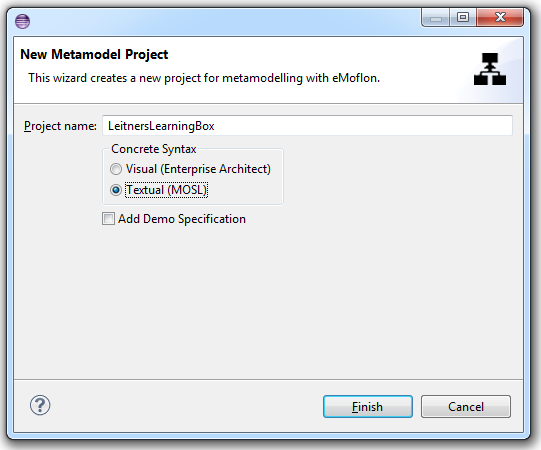
\includegraphics[width=0.6\textwidth]{eclipse_newMetamodelTextPlain}
	\caption{Create a new concrete metamodeling project}
	\label{fig:new_project}
\end{figure}

% Since both sections are talking about the same thing, shoud we write a paragraph and define them both at the same time?
\item[$\blacktriangleright$] Following 
\marginpar{\emph{Meta-metamodel}} the same ``everything is an object'' princicple that's been established in the Object-oriented Paradigm, in metamodeling, everything is a model! This
\marginpar{\emph{Modelling language}}  includes those that define even small parts of languages - they too must be models. This means the metamodel(s) conform to some \emph{meta-metamodel}, 
\marginpar{\emph{meta-language}}which then defines a \emph{(meta)modelling language}\footnote{Other modelling languages include MOF, UML, and Kermeta.} or \emph{meta-language}. All of this together is called \emph{unification}\marginpar{\emph{Unification}}, the bringing together of two or more things so they become a single unit - your program! When metamodeling with eMoflon, we support \emph{Ecore} as the modeling language which define the \emph{EClass} and \emph{EReference} types.

\item[$\blacktriangleright$] Expand the project as deep as it goes. Your Package explorer may look different than ours, displayed in figure~\ref{fig:expanded_folders}, depending on whether you completed the Demo in Part I. In an effort to keep things clear as possible, we have removed them from our workspaces, but recommend keeping them for future reference.

\begin{figure}[htbp]
	\centering
  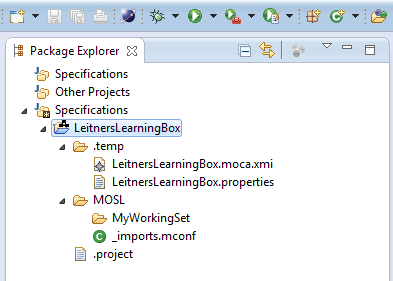
\includegraphics[width=0.5\textwidth]{eclipse_foldersExpanded}
	\caption{Expanded project files}
	\label{fig:expanded_folders}
\end{figure} 

\item[$\blacktriangleright$] You can see two folders - \texttt{.temp}, and \texttt{MOSL} - and one subfolder, \texttt{MyWorkingSet}, all within the \texttt{Specifications} node\footnote{for detailed review on the explorer structre, look over Part I}. We're most insterested in \texttt{MyWorkingSet}, which stores the collection of files and  \emph{unifies} everything we need for Leitner's Box. 

\item[$\blacktriangleright$] Right click on your current workspace folder, \texttt{MyWorkingSet}, and create a new subfolder. Name it \texttt{LearningBoxLanguage}. This is now the container for all your modelling files!


\item[$\blacktriangleright$] Right click on \texttt{LearningBoxLanguage} and create your first eclass model by going to ``New/EClass.'' Name it \texttt{Box}.

\item[$\blacktriangleright$] The class editor should have automatically appeared. Currently, it's empty; Lets add the first two EAttributes of our program, \texttt{name} and \texttt{stringRep}. Both are \texttt{EString} types (fig~\ref{fig:boxDeclaration}).

\begin{figure}[htbp]
	\centering
  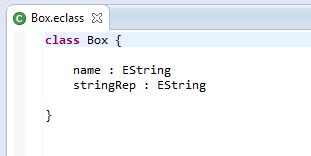
\includegraphics[width=0.5\textwidth]{eclipse_classBoxDeclaration}
	\caption{Newly created box class}
	\label{fig:boxDeclaration}
\end{figure} 

\item[$\blacktriangleright$] Create two more classes in your model the same way, \texttt{Partition} and \texttt{Card}. 

\item[$\blacktriangleright$] In \texttt{Partition}, add two \texttt{EInt} datatypes, \texttt{index} and \texttt{partitionSize}. 

\item[$\blacktriangleright$] In \texttt{Card}, create three \texttt{EString}s, \texttt{back}, \texttt{face} , and \texttt{partitionHistory}.

\item[$\blacktriangleright$] If you've done everything correctly, the key areas of your workspace should now resemble figure~\ref{fig:workspaceClassAttributes}.

\begin{figure}[htbp]
	\centering
  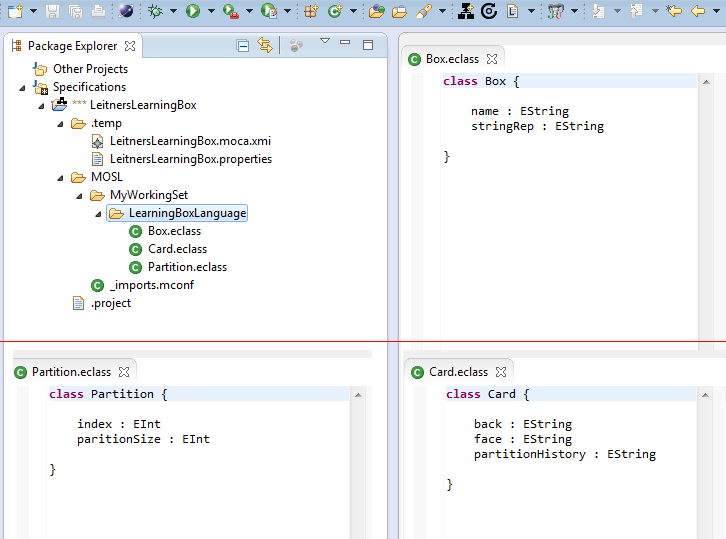
\includegraphics[width=0.9\textwidth]{eclipse_workspaceClassesAttributes}
	\caption{Declaration of classes and attributes}
	\label{fig:workspaceClassAttributes}
\end{figure} 

\item[$\blacktriangleright$] Now, lets add some references. MOSL supports two reference types - a \emph{contained reference} and a \emph{simple reference}. Both automatically update the other element involved in the reference automatically, which means you only have to declare a direction once.

\item[$\blacktriangleright$] Activate the \texttt{Card} editor and add a simple reference named \texttt{cardContainer} with a multiplicity of zero to one, of type \texttt{Partition} (fig.~\ref{fig:cardReference}). This means that a single card can belong to a maximum of 1 partition.

\begin{figure}[htbp]
	\centering
  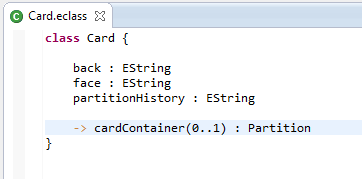
\includegraphics[width=0.5\textwidth]{eclipse_cardReference}
	\caption{Creating a \emph{simple reference} in Card}
	\label{fig:cardReference}
\end{figure} 

\item[$\blacktriangleright$] Now add a \emph{container reference} to \texttt{Partition}. Name it \texttt{card}, and allow it to hold an unlimited amount of cards.

\item[$\blacktriangleright$] Congratulations, you just built your first \emph{Bidirectional EReference}! In essence, you have now set up a relation that allows a potentially infinite amount of item \texttt{card} to be stored in a partition container, and restricts that \texttt{containedCard} to only \emph{one} partition.

\item[$\blacktriangleright$] Now, lets create another bidirectional association between \texttt{Partition} and \texttt{Box}. If you think about it, it's really not all that different than the relation between \texttt{Partition} and \texttt{Card}. In fact, it's not different at all! A \texttt{Box} should be able to hold an unlimited amount of partitions, but a \texttt{Partition} should only be allowed to belong to zero or one boxes. Name the two new relations \texttt{containedPartition}, and \texttt{box}. 

\item[$\blacktriangleright$] Your classes should now closely resemble figure~\ref{fig:allReferences}.


\begin{figure}[htbp]
	\centering
  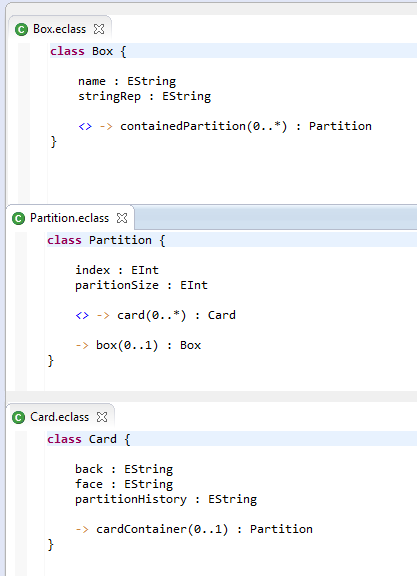
\includegraphics[width=0.5\textwidth]{eclipse_workspaceReferences}
	\caption{The Completed Bidirectional EReferences.}
	\label{fig:allReferences}
\end{figure} 


\item[$\blacktriangleright$] The next step is to set up two relations between \texttt{Partition} and itself, so it can shift between the previous and next partition in the box. Create two new simple references, named \texttt{previous}, and \texttt{next}. Allow them to have a maximum of 1 link each. If you've done everything correctly, your \texttt{Partition} class should now resemble figure~\ref{fig:partitionReferences}.

\begin{figure}[htbp]
	\centering
  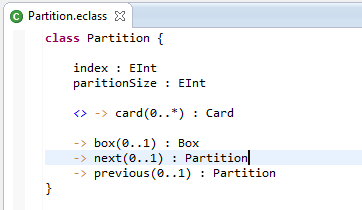
\includegraphics[width=0.5\textwidth]{eclipse_partitionReferences}
	\caption{All references in Partition}
	\label{fig:partitionReferences}
\end{figure} 

\item[$\blacktriangleright$] All of our references are now set up! To see how all of this is depicted visually, check out figure~\ref{fig:ereferences_all} in section~\ref{sec:staticAbstract}.

\pagebreak

\item[$\blacktriangleright$] You're almost done setting up the static structure of your model! The last thing we need to do is to make the program \emph{do} something. After all, what good is a program that only stores attributes and references?

\item[$\blacktriangleright$] In a language, the rules that describe a system's behavior and how it evolves over time, or reacts to external stimulus, are collectively referred to as \emph{Dynamic Semantics}. Although these could be defined as a separate set of \emph{model transformations}, we take a holistic approach and advocate integrating these transformations directly in the metamodel as operations. This falls within the OO Paradigm, and is quite natural in may ways.

\item[$\blacktriangleright$] Lets start to set up our these operations by declaring their \emph{signatures}, starting with the \texttt{Partition} class. We want a partition to be able to do three things: check the answer on a \texttt{card} with a guess and return a true/false value, remove a specific card, or empty itself of all cards to reset. 

\item[$\blacktriangleright$] Start with the \texttt{empty} method - it won't need any parameters, and it doesn't need to return anything. Declare this via a \texttt{empty():void} command\footnote{If you're having difficulty remembering the syntax for MOSL, feel free to review \mbox{\texttt{Part I}}} .

\item[$\blacktriangleright$] Create two more functions for \texttt{Partition} the same way. We'll need a \texttt{removeCard} method that accepts and returns a \texttt{Card}, as well as a EBoolean \texttt{check} method that accepts a \texttt{Card} and an \texttt{EString} guess. Your partition class should now resemble figure~\ref{fig:partitionMethods}.

\begin{figure}[htbp]
	\centering
  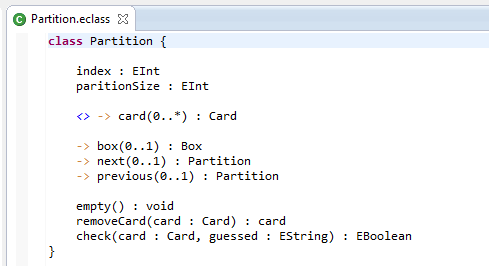
\includegraphics[width=0.6\textwidth]{eclipse_partitionMethods}
	\caption{The completed \texttt{Partition} class}
	\label{fig:partitionMethods}
\end{figure}

\item[$\blacktriangleright$] What needs to be done in the \texttt{Card} class? Well, in order to check the card, we'll need to be able to look at the flip side. We'll also need to print whatever is on the current side. Create two void functions, \texttt{invert} and \texttt{printCard}.

\pagebreak

\item[$\blacktriangleright$] Finally, what do we need to do with the largest object in our model, the \texttt{Box}? In summary, we want to allow a \texttt{Box} to:

\begin{description}
	{\small
  \item[\texttt{determineNextSize():EInt }] find out how big the upcoming partition is
  \item[\texttt{grow():void}] increase in size (to allow more partitions)
  \item[\texttt{toString():EString}] display all current content within it
  \item[\texttt{addToStringRep(card:Card):void}] not sure yet
  }
\end{description}


\item[$\blacktriangleright$] Your workspace should now resemble figure~\ref{fig:workspaceMethods}.
\begin{figure}[htbp]
	\centering
  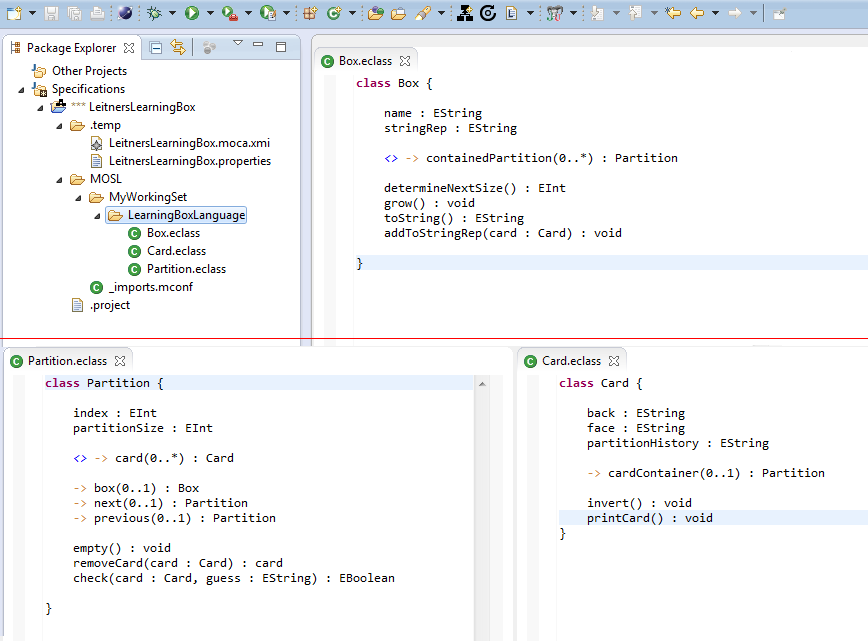
\includegraphics[width=0.95\textwidth]{eclipse_workspaceMethods}
	\caption{Completed Method Signatures}
	\label{fig:workspaceMethods}
\end{figure}


\item[$\blacktriangleright$] Congratulations! You've \emph{almost} completeley modeled Leitner's Learning Box using a concrete, textual syntax! To see how this looks in visually in a class diagram, check out figure~\ref{fig:metamodel_complete} from section~\ref{sec:staticAbstract}.

\item[$\blacktriangleright$] Let's review our model so far. We have modeled a \texttt{Box} which that can hold an unknown number of \texttt{Partitions}, who can in turn, store an unknown number of \texttt{Card}s. A \texttt{Partition} is identified by its' \texttt{index} value and can, but does not \emph{need} to, have a previous and next \texttt{Partition}. Finally, each card has a front, back, and unique history that the user (you!) can review to see that card's successes and failures. A card can belong to exclusively one partition at a time.

\item[$\blacktriangleright$]The very last thing we need to do now is conduct a build and generate the required \texttt{.genmodel} and \texttt{.ecore} files. Beside the \texttt{New Metamodel} button on the toolbar, you'll notice that there is a circular arrow button that offers to ``Build (without cleaning).'' %explain this here?

\item[$\blacktriangleright$] If you've done everything correctly, a new \texttt{MyWorkingSet} node should have appeared, and your entire expanded Package Explorer should resemble figure~\ref{fig:builtModel}.

\begin{figure}[htbp]
	\centering
  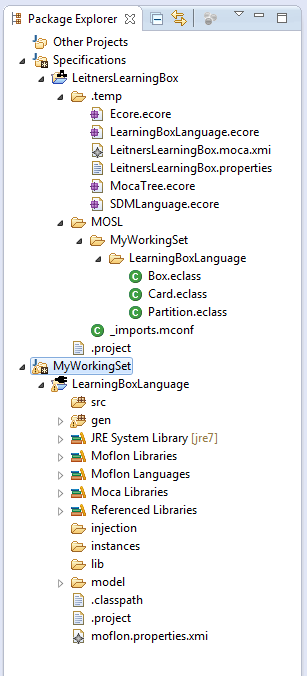
\includegraphics[width=0.5\textwidth]{eclipse_finalPackageExplorer}
	\caption{Final Static Semantics Project Structure}
	\label{fig:builtModel}
\end{figure}

\item[$\blacktriangleright$] Examine the generated files in \texttt{gen} folder, especially the default implementation for all methods that just throw an \texttt{OperationNotSupported} exception. We shall see in later handbook parts that the EMF code generator actually supports injecting hand-written implementation of methods into generated methods and classes. With eMoflon however, we can model a large part of the dynamic semantics and only need to implement small helper methods, such as those for string manipulation, by hand.

\item[$\blacktriangleright$] Finally, you can see that your two metamodels have been created and placed in the \texttt{model} folder. Together, they form everything the EMF needs to generate your program. In fact, if you like, instead of viewing your \texttt{.ecore} model in a tree diagram, you can request eclipse to build a visual diagram with its built-in visual modeler! Right click on \texttt{LearningBoxLanguage.ecore} and select ''Initilalize Ecore Diagram File.''

\fancyfoot[R]{ $\triangleright$ \hyperlink{validation tex}{Next step} }

\item[$\blacktriangleright$] You're all done! We encourage you to review section~\ref{sec:staticAbstract} and observe how this same project is crafted using visual tools. Compare the differences between modeling the three classes in a separate, abstract program and exporting to eclipse in order to build them, versus modeling and building all within eclipse. Which do you find easier to work with?

\end{itemize}